\begin{figure*}[t]
     \centering
     % \textbf{\rotatebox{90}{CNN$\,\;$}}
     \begin{subfigure}[b]{0.24\textwidth}
         \centering
         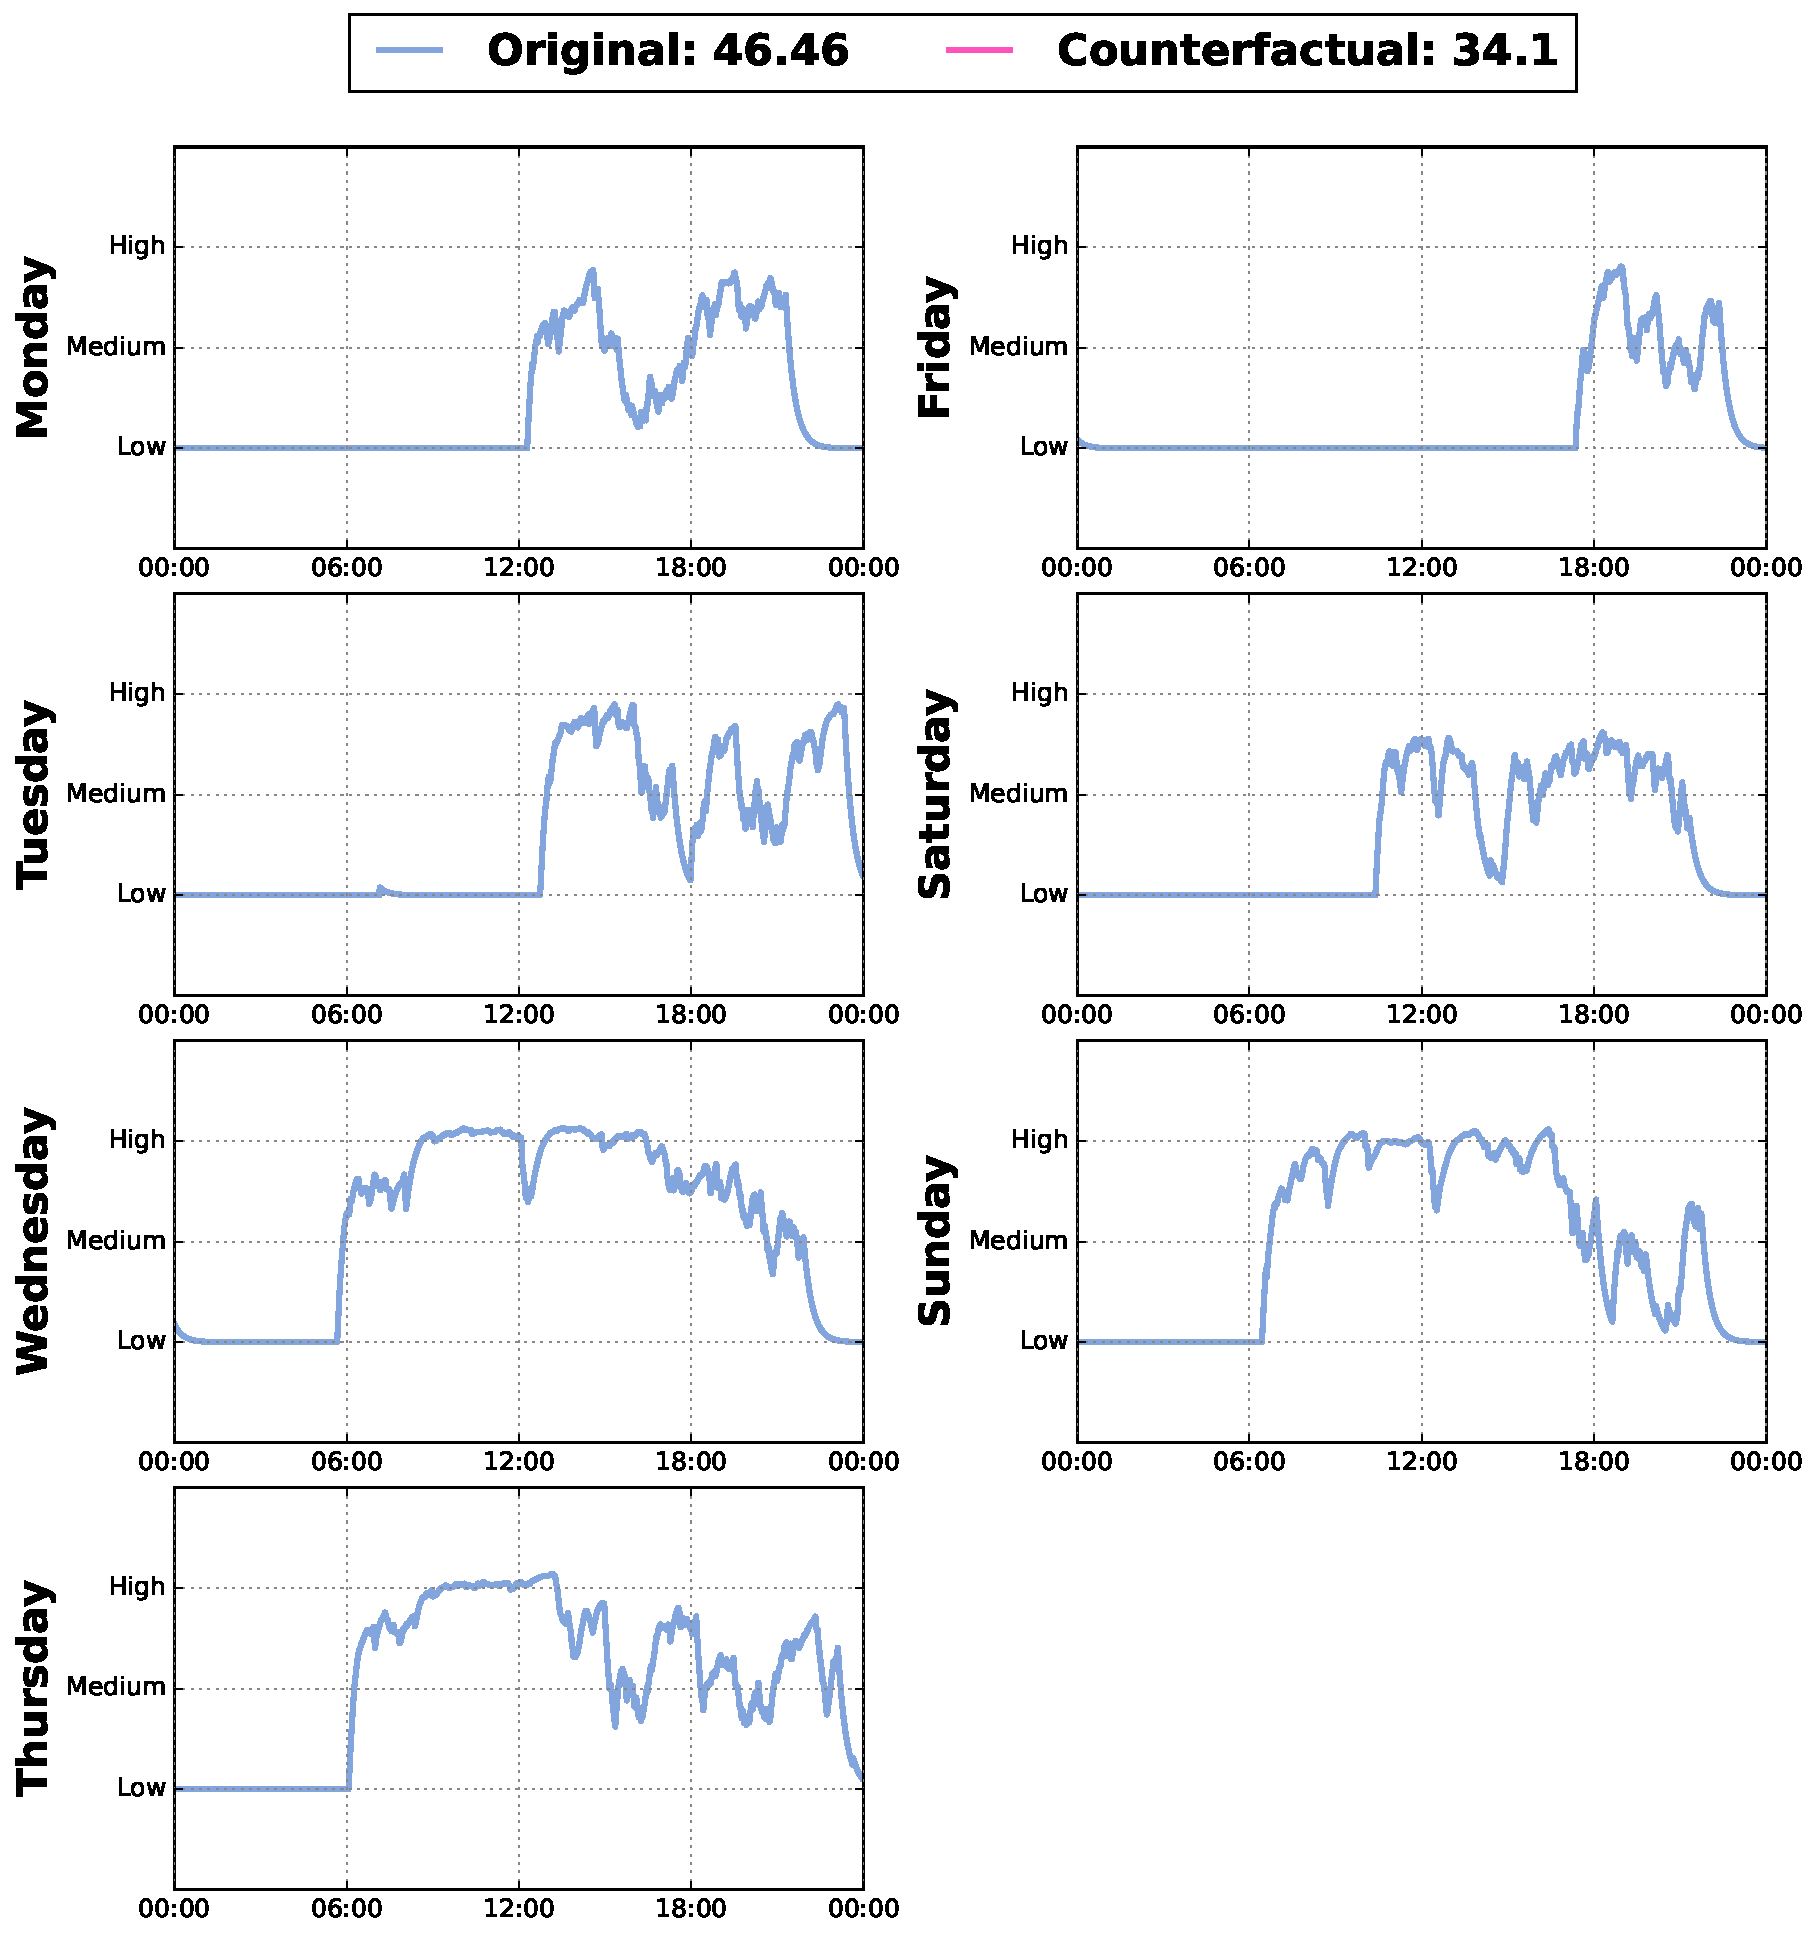
\includegraphics[width=\textwidth]{images/6306/0_6306_TCN_Wachter_cf.pdf}
         \caption{\gls{wachter} Counterfactual}
         \label{fig:cf:wachter}
     \end{subfigure}
     \hfill
     \begin{subfigure}[b]{0.24\textwidth}
         \centering
         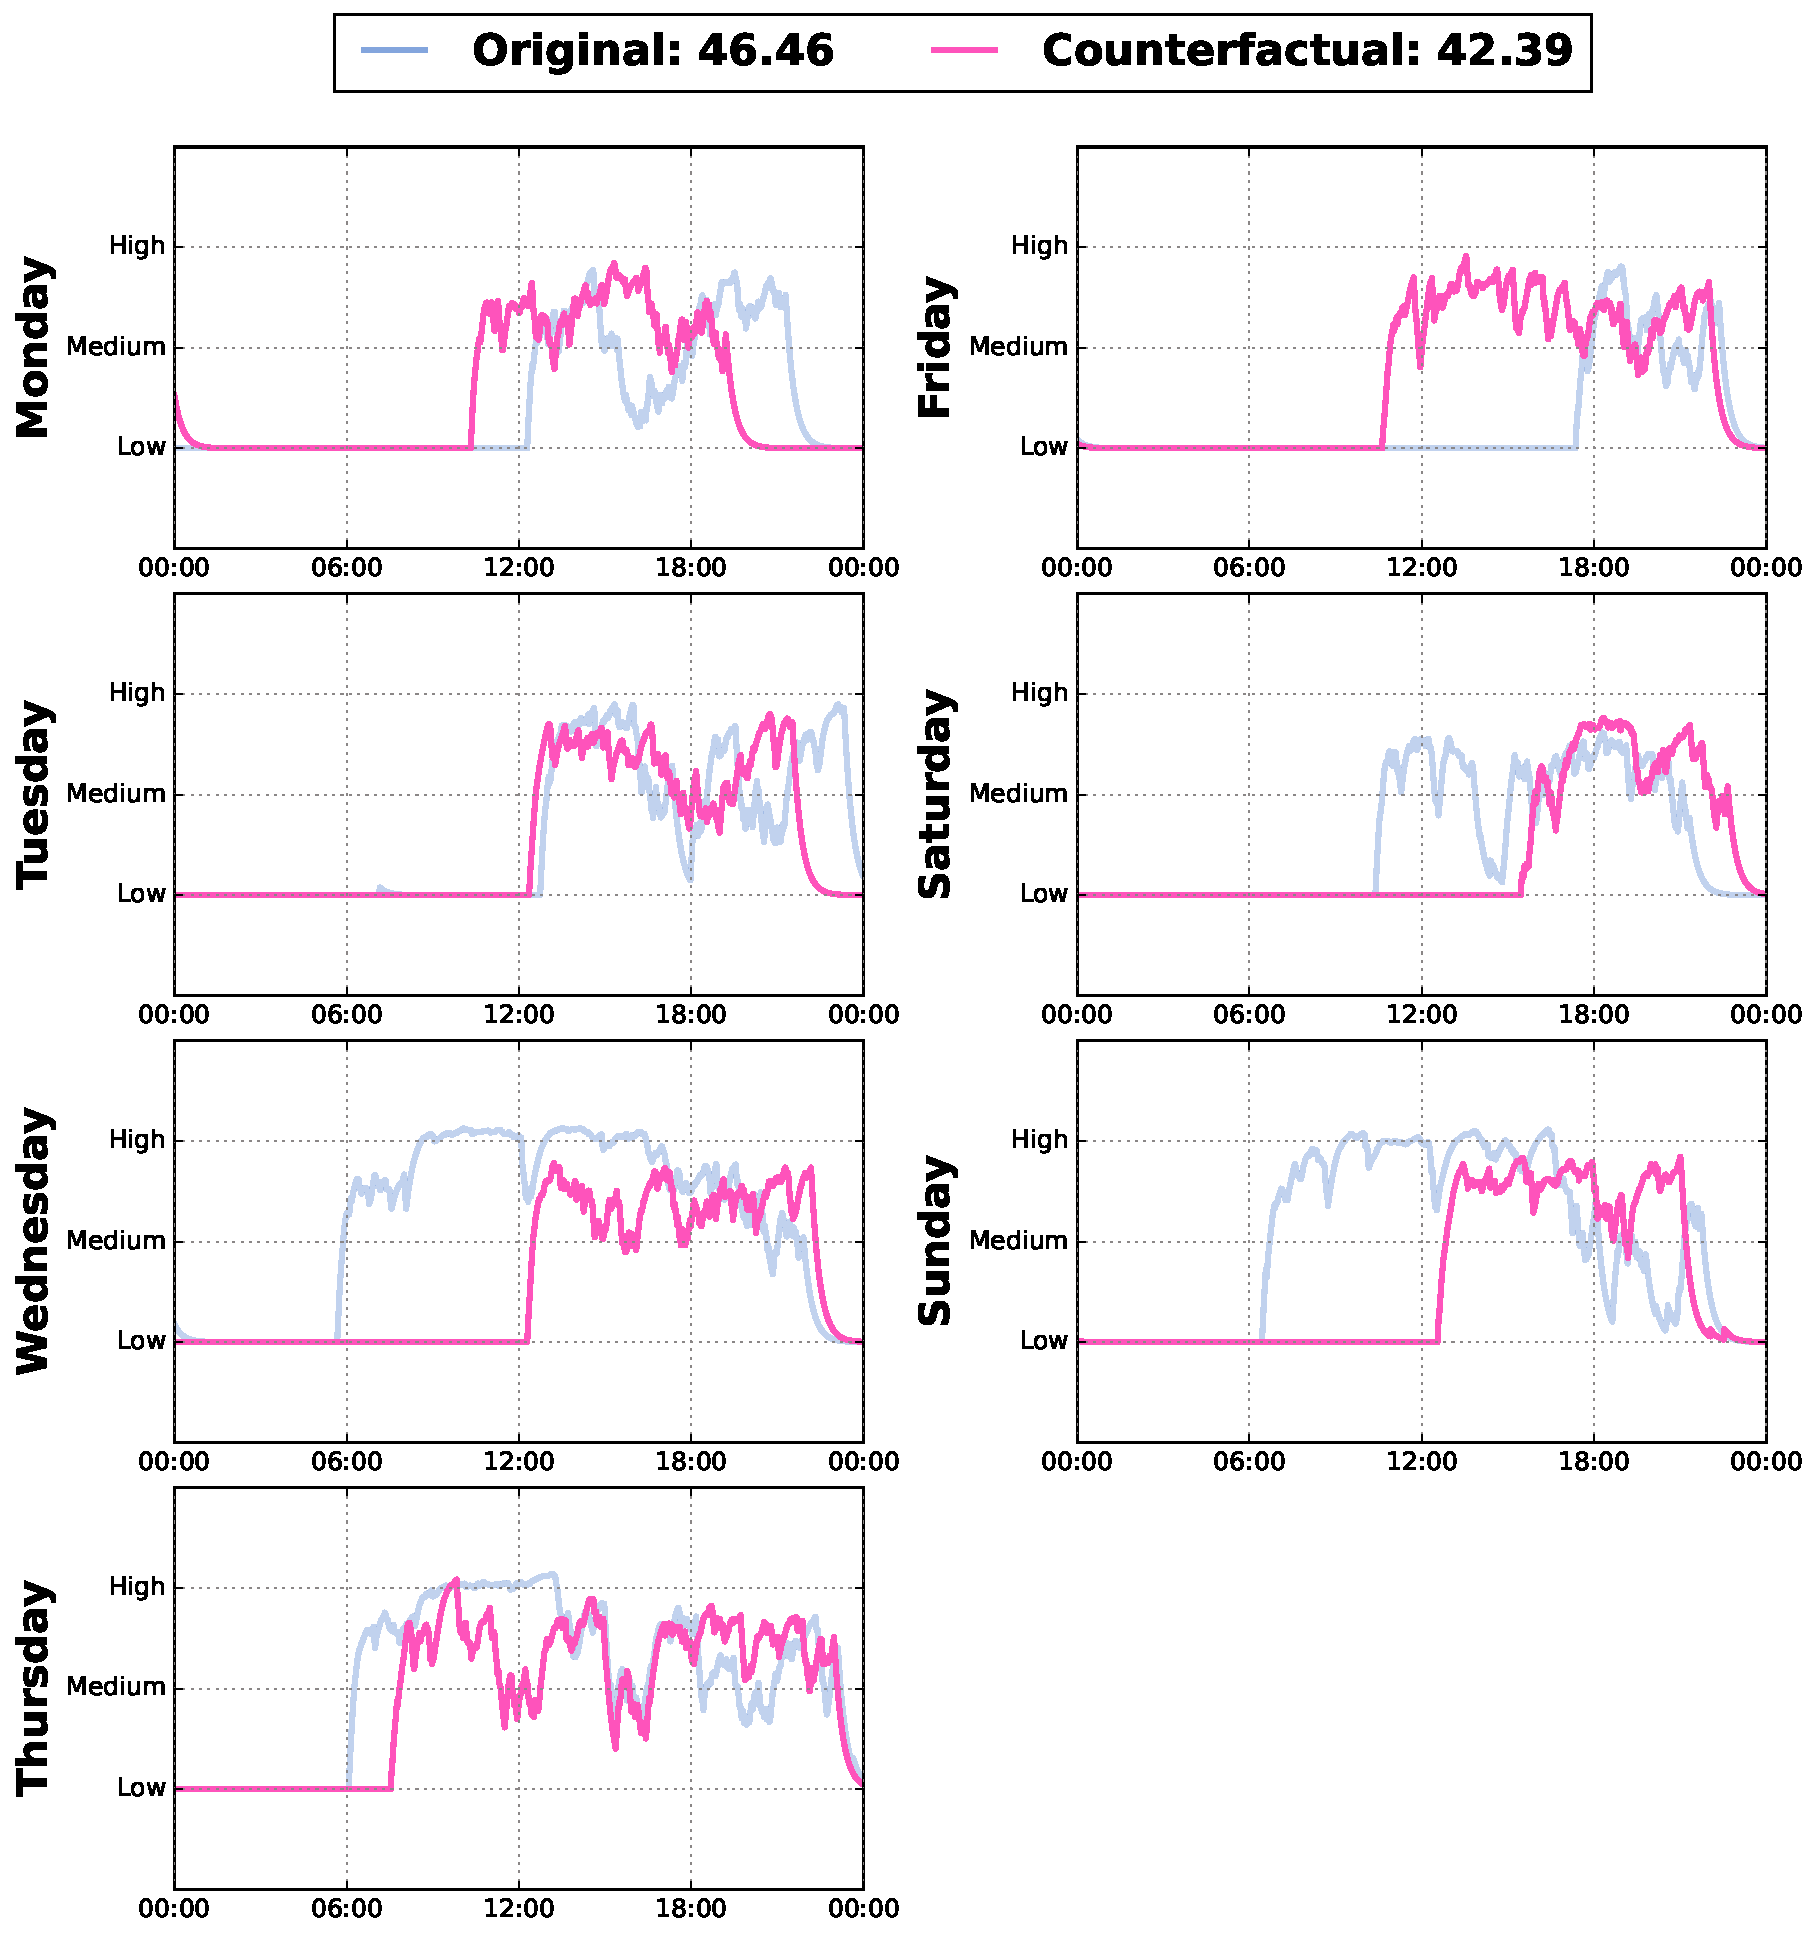
\includegraphics[width=\textwidth]{images/6306/4_6306_TCN_NUN_cf.pdf}
         \caption{NUNR Counterfactual}
         \label{fig:cf:nun}
     \end{subfigure}
     \hfill
     \begin{subfigure}[b]{0.24\textwidth}
         \centering
         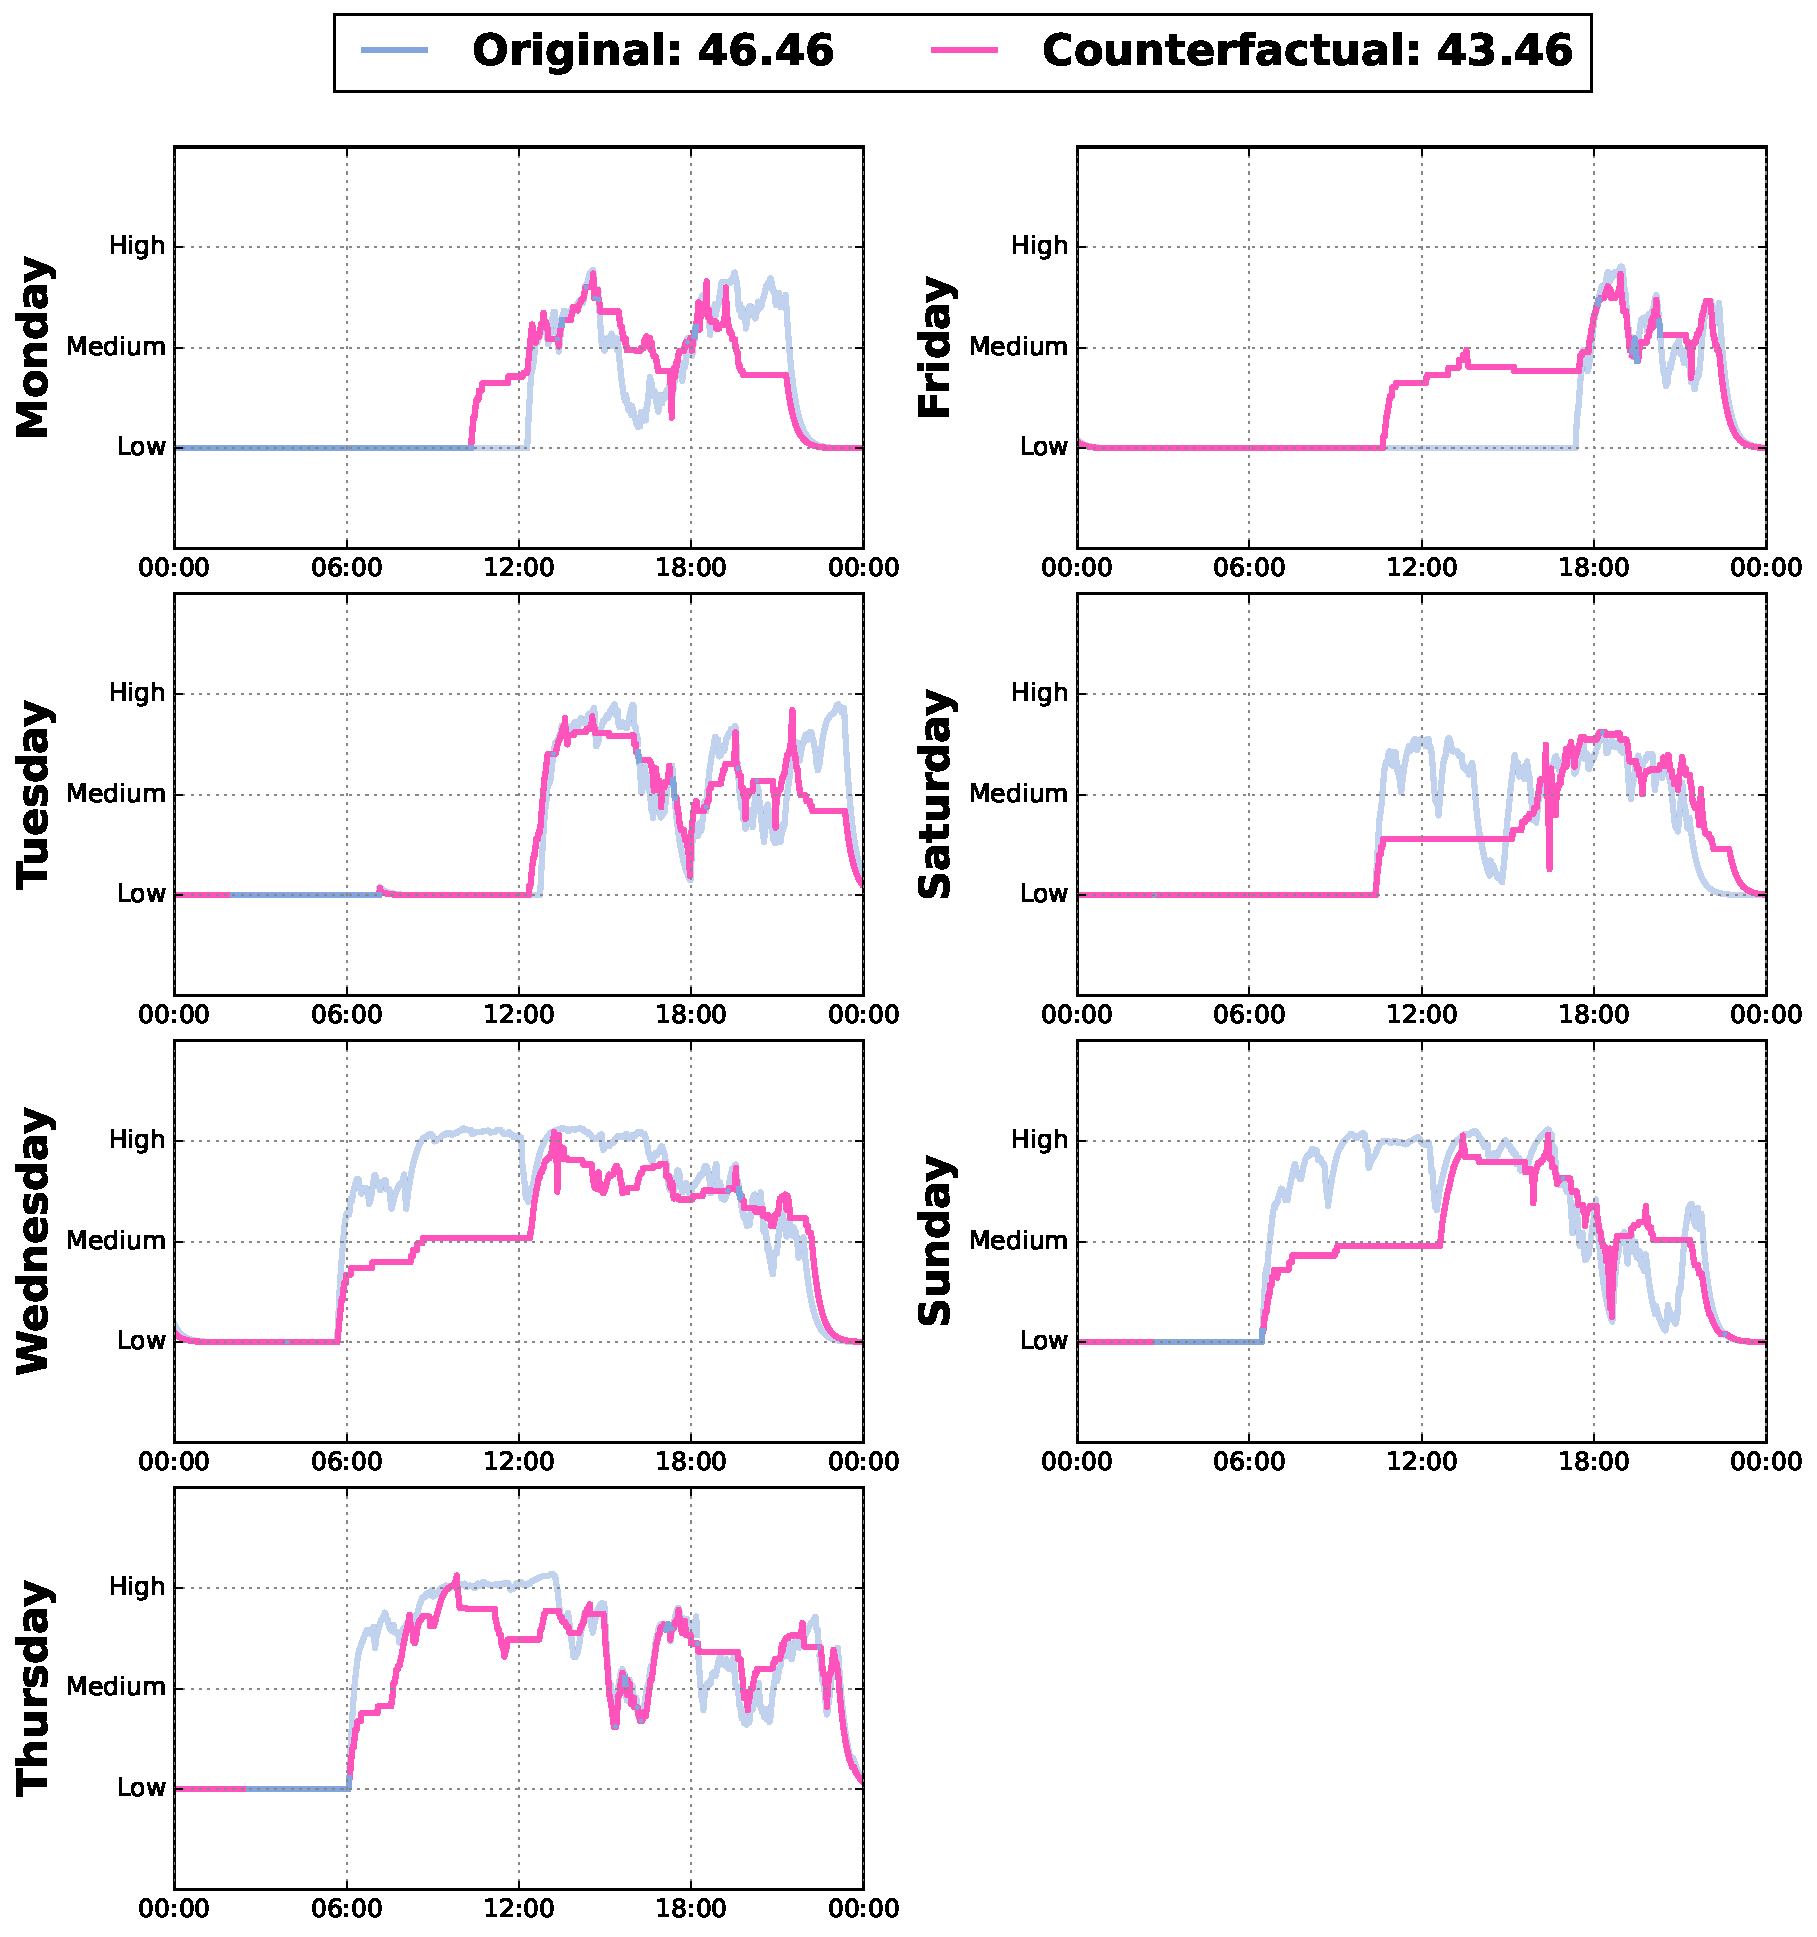
\includegraphics[width=\textwidth]{images/6306/1_6306_TCN_DBA_cf.pdf}
         \caption{DBAR Counterfactual}
         \label{fig:cf:dba}
     \end{subfigure}
    \hfill
     \begin{subfigure}[b]{0.24\textwidth}
         \centering
         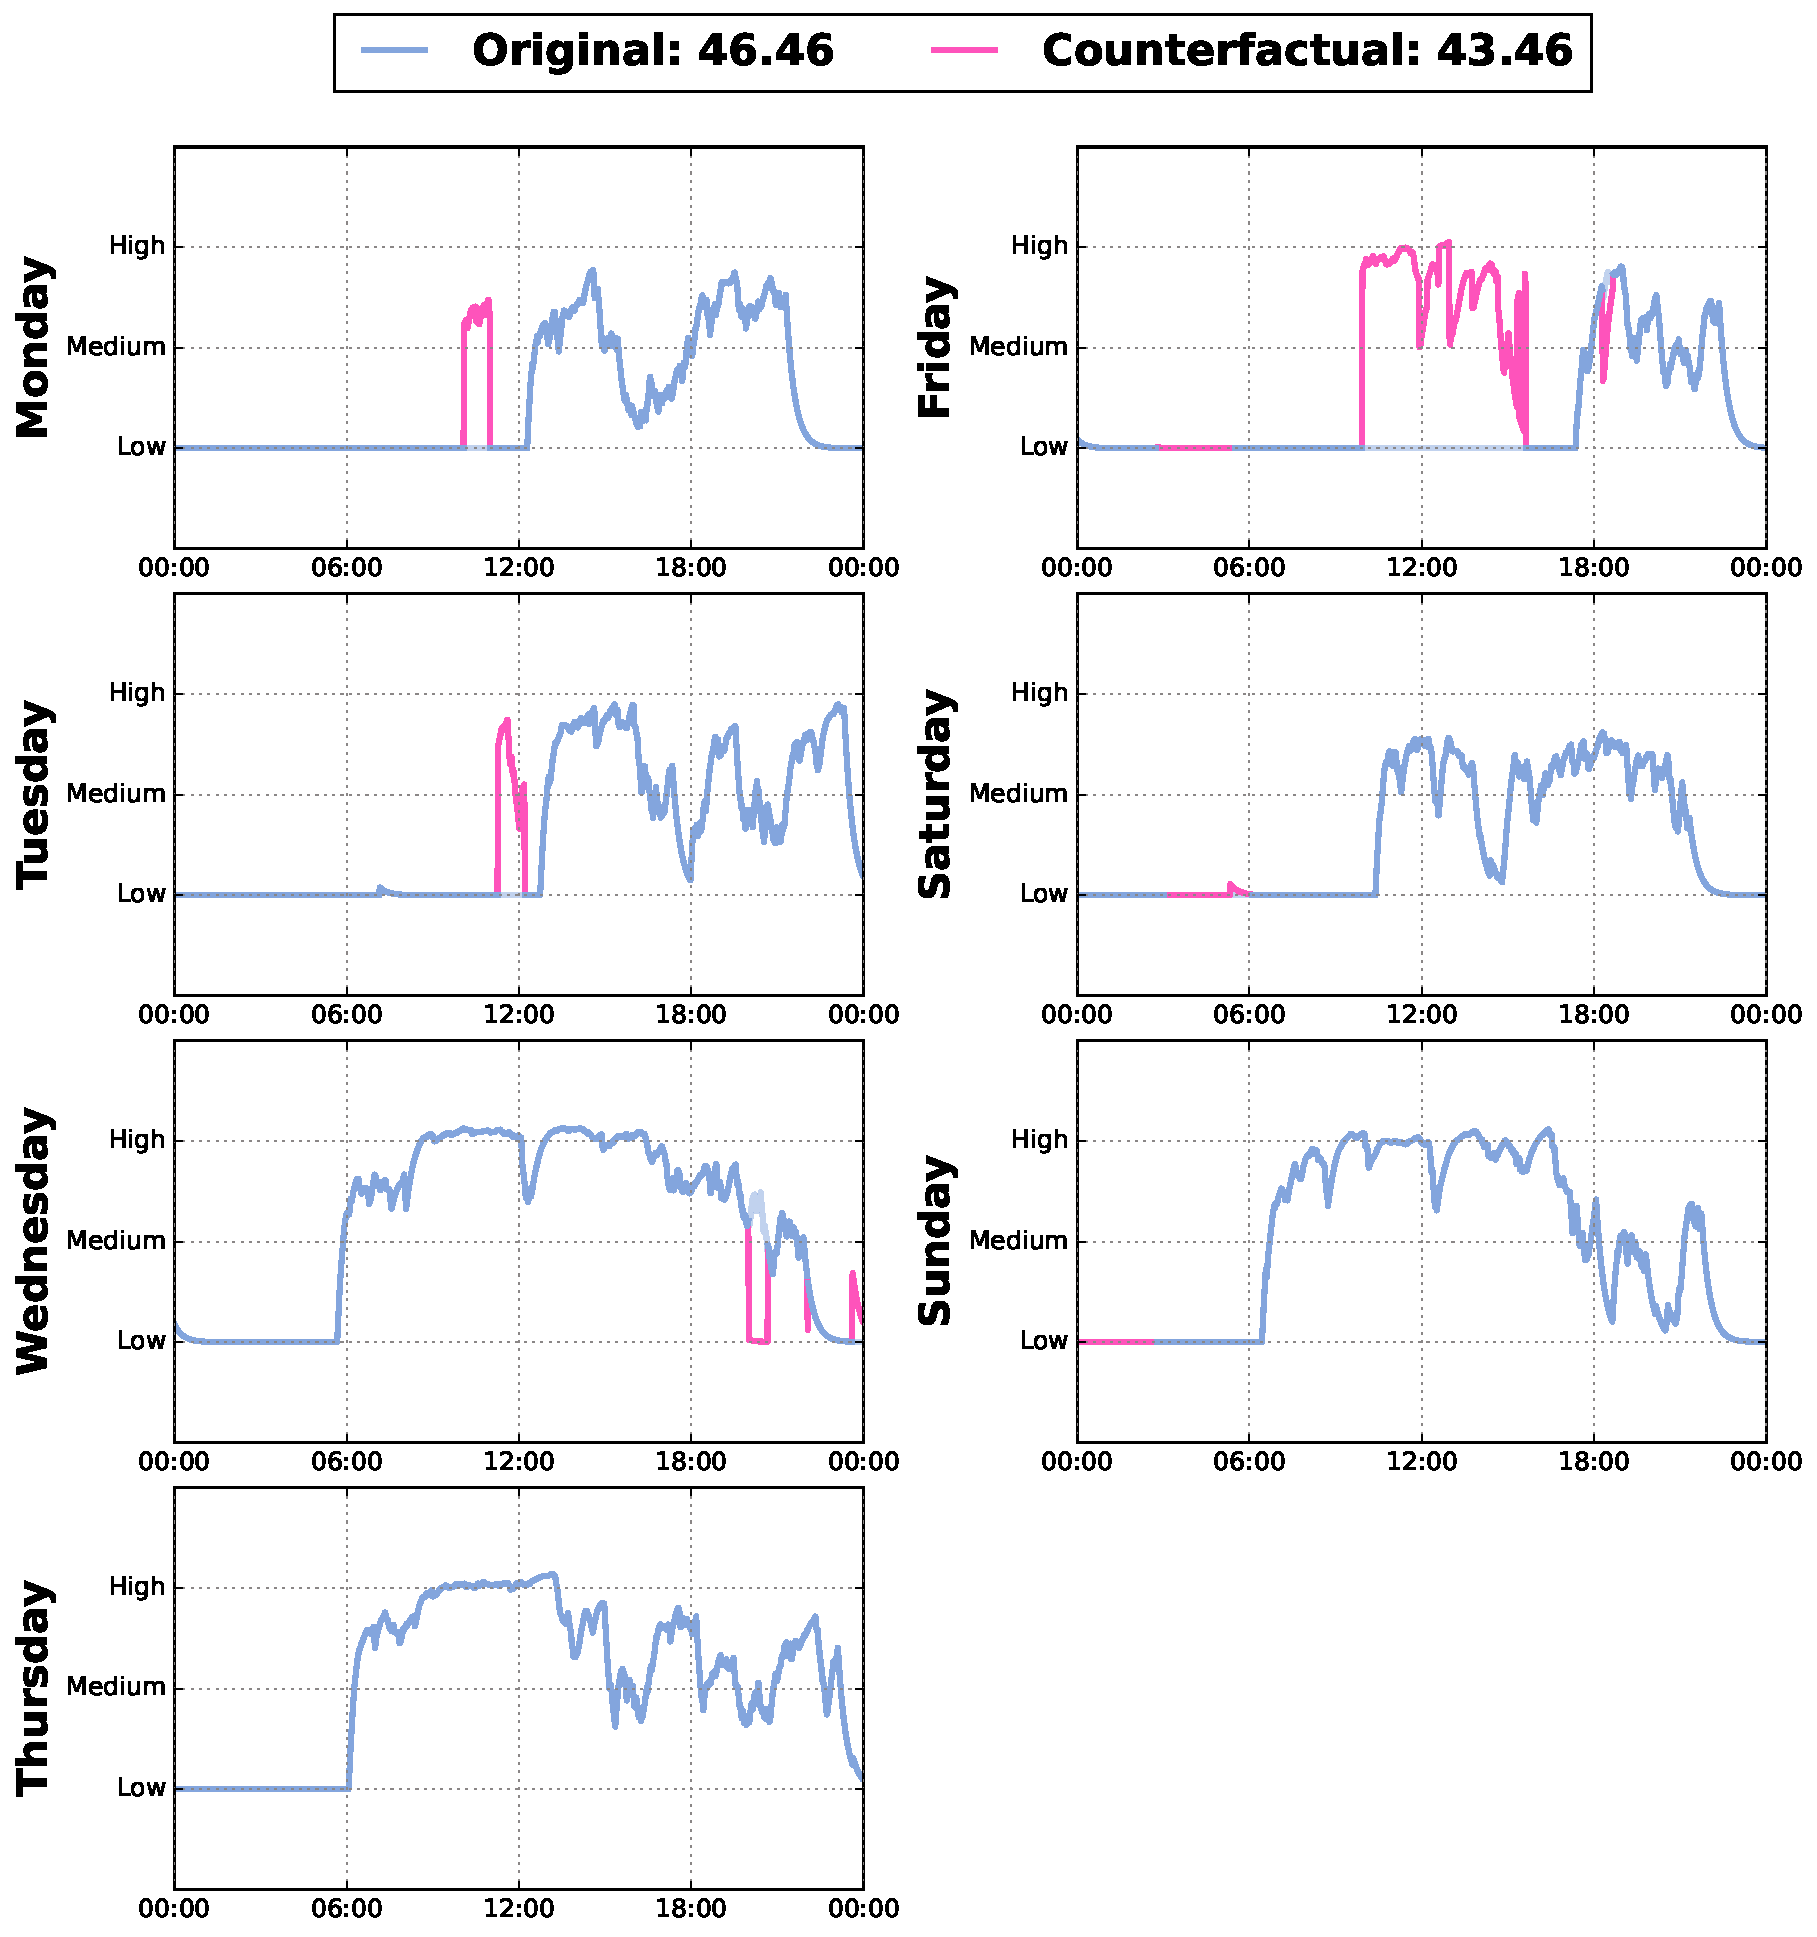
\includegraphics[width=\textwidth]{images/6306/2_6306_TCN_TSEvo_cf.pdf}
         \caption{TSEvoR Counterfactual}
         \label{fig:cf:tsevo}
     \end{subfigure}

          \begin{subfigure}[b]{0.24\textwidth}
         \centering
         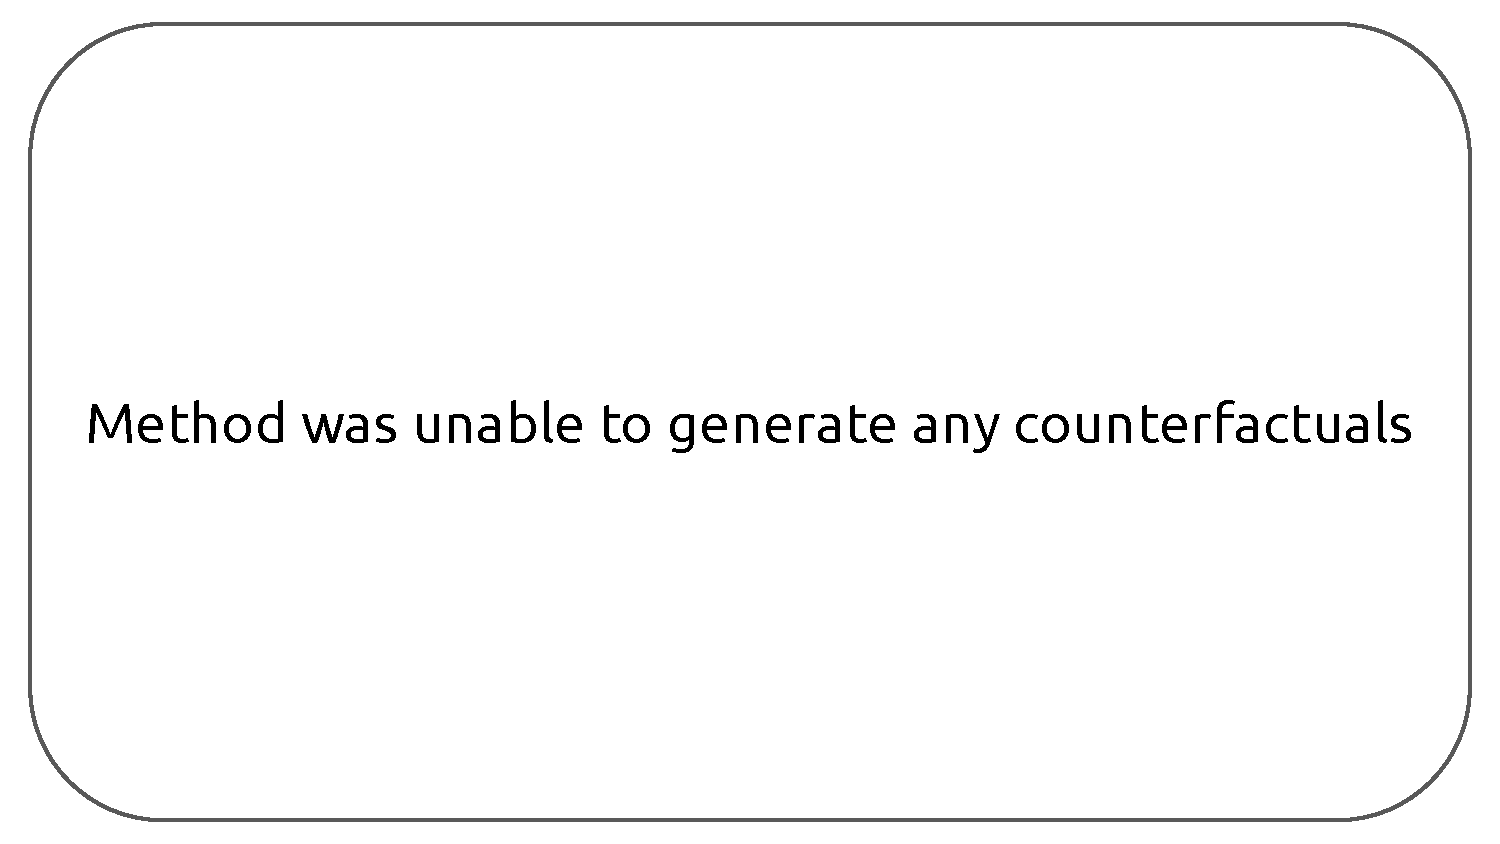
\includegraphics[width=\textwidth]{images/6306/0_6306_TCN_Wachter_reco.pdf}
         \caption{\gls{wachter} Recommendations}
         \label{fig:reco:wachter}
     \end{subfigure}
     \hfill
     \begin{subfigure}[b]{0.24\textwidth}
         \centering
         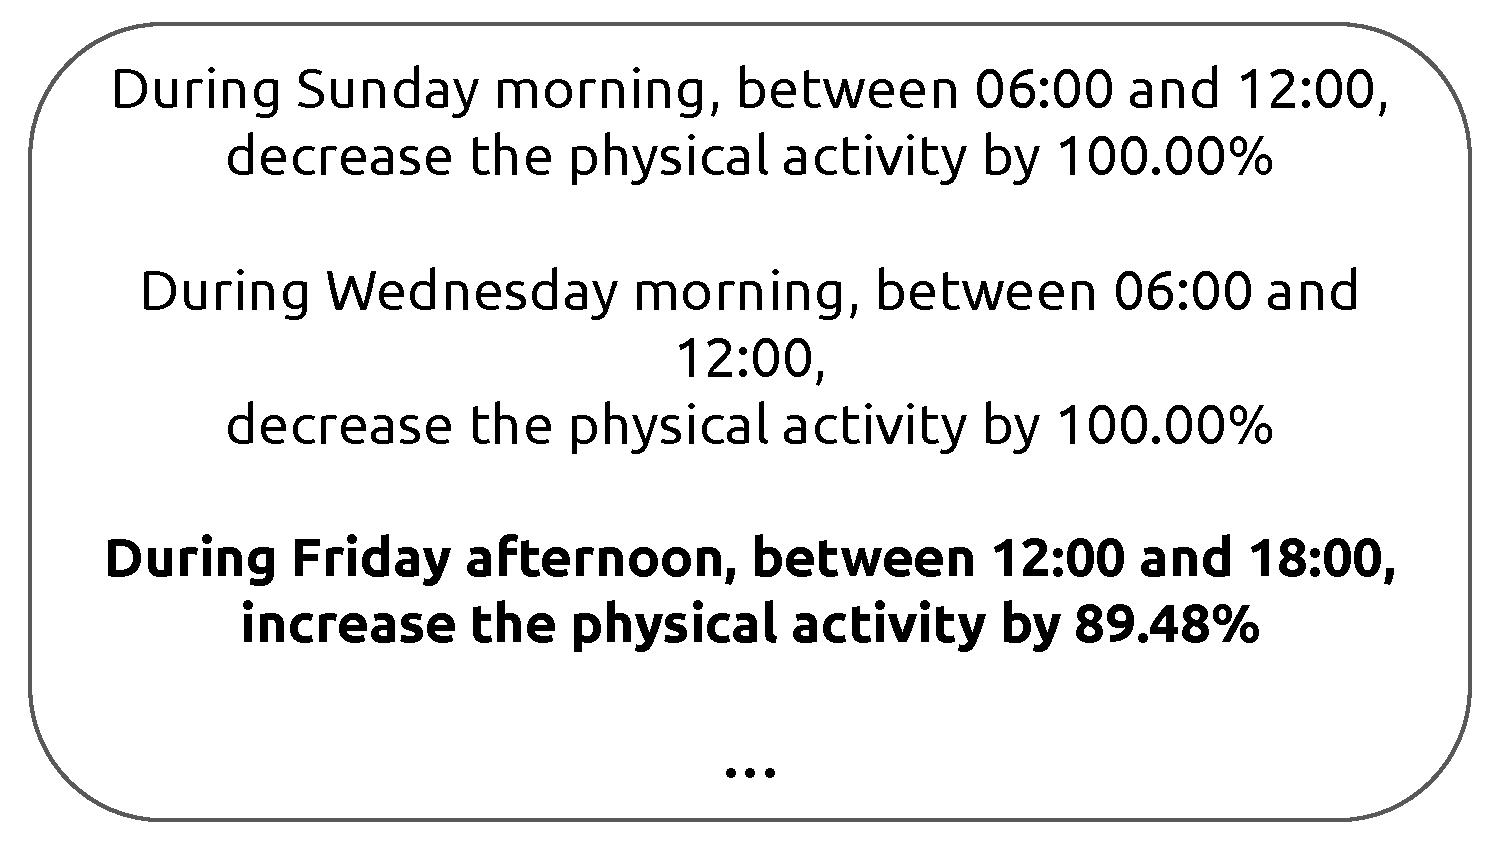
\includegraphics[width=\textwidth]{images/6306/4_6306_TCN_NUN_reco_bold.pdf}
         \caption{NUNR Recommendations}
         \label{fig:reco:nun}
     \end{subfigure}
     \hfill
     \begin{subfigure}[b]{0.24\textwidth}
         \centering
         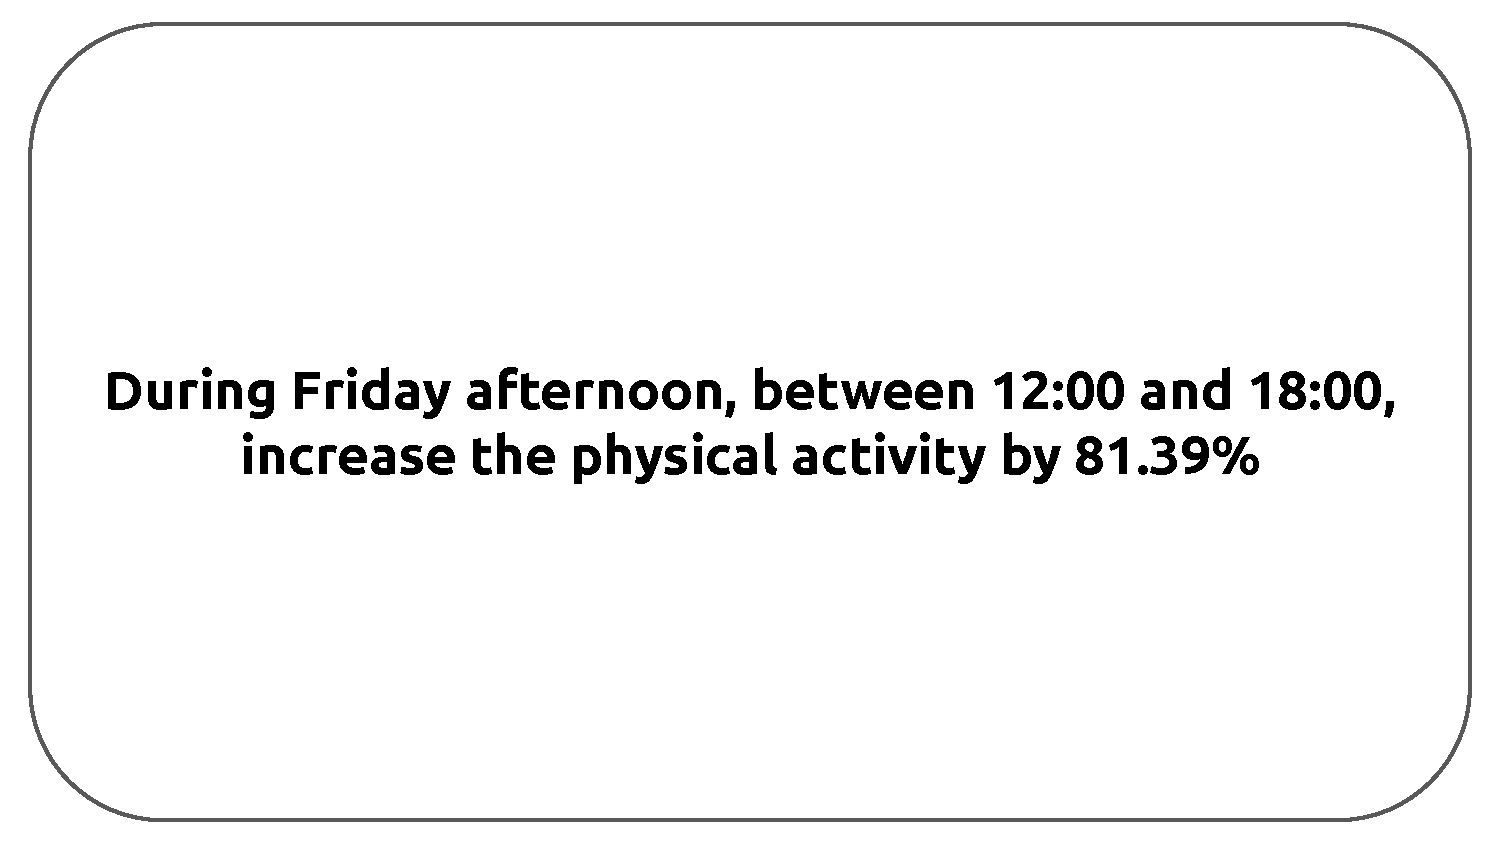
\includegraphics[width=\textwidth]{images/6306/1_6306_TCN_DBA_reco_bold.pdf}
         \caption{DBAR Recommendations}
         \label{fig:reco:dba}
     \end{subfigure}
    \hfill
     \begin{subfigure}[b]{0.24\textwidth}
         \centering
         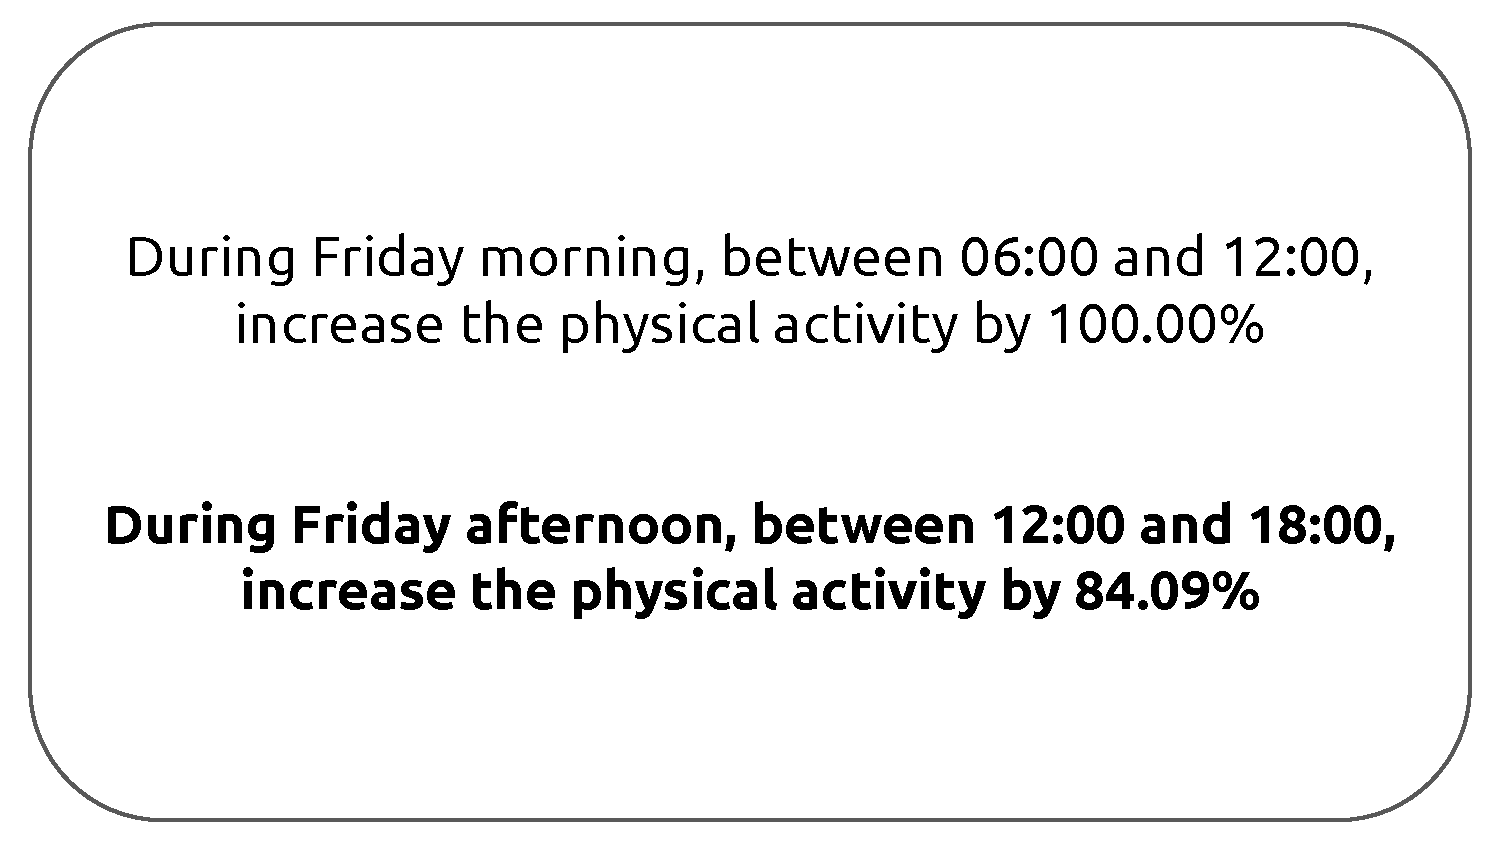
\includegraphics[width=\textwidth]{images/6306/2_6306_TCN_TSEvo_reco_bold.pdf}
         \caption{TSEvoR Recommendations}
         \label{fig:reco:tsevo}
     \end{subfigure}

    \caption{Example of time series counterfactuals (pink line) of an input time
series (blue line) for the biological estimation problem, where, given a threshold $\varepsilon=3$, the counterfactual modifies the original activity so the \gls{dl} model predicts a smaller biological age. Each plot represents a different counterfactual technique, and each corresponding text recommendation is listed below the plot. Common recommendations are in bold.}
    \label{fig:quali-eval}
\end{figure*}